\section{Experiments}
\label{sec:experiments}
\eeTable

\begin{figure*}[t]
\centering
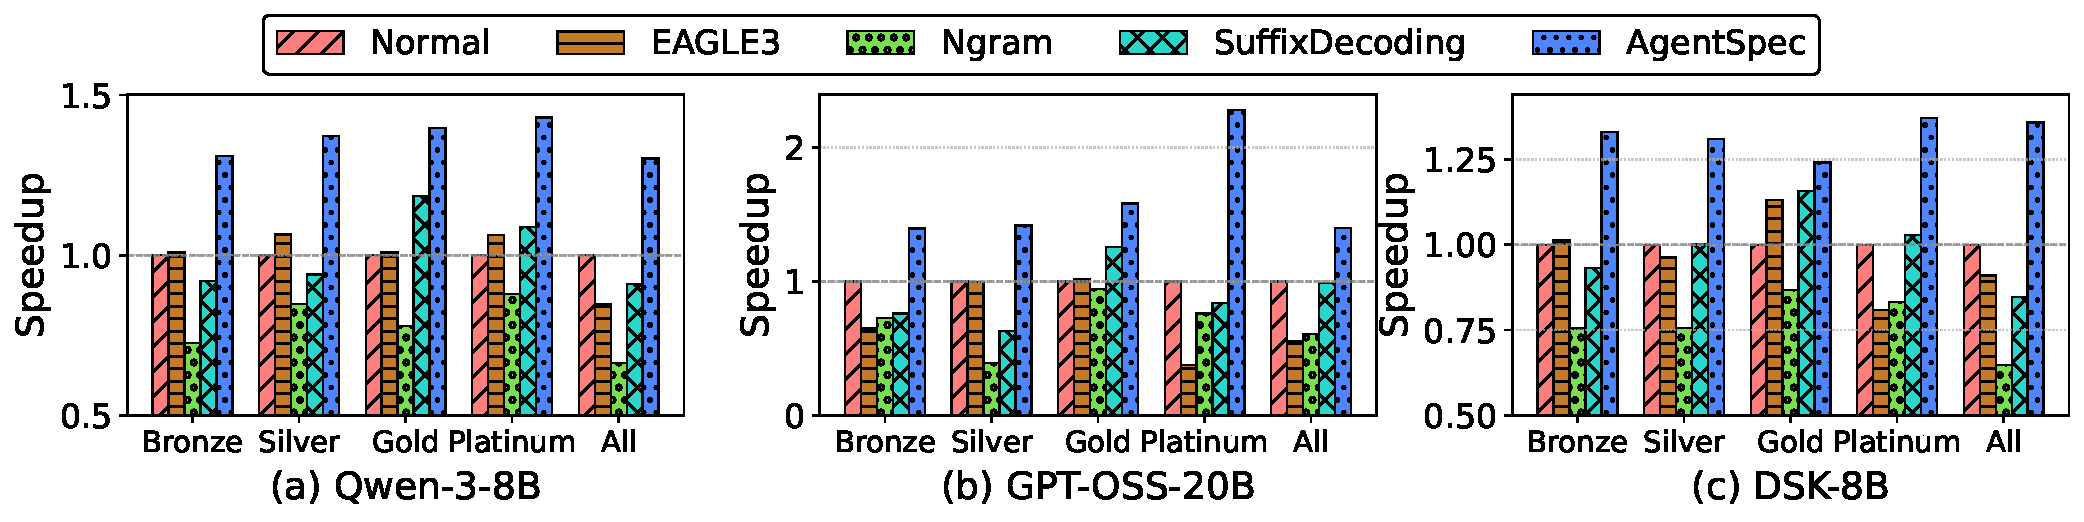
\includegraphics[width=0.98\textwidth]{Figures/e2e_throughput.pdf}
\vspace{-3mm}
\caption{Speedup in terms of Goodput (token/s) for \sysname and baselines compared with normal autoregressive decoding on all subsets in USACO dataset with Code Generation Agent implemented by Reflexion agentic workflow on three different models.}
\vspace{-3mm}
\label{fig:e2e_subset}
\end{figure*}

\subsection{Experimental Setups}
\label{subsec:setup}

\noindent\textbf{Baselines.} We compare \sysname against two groups of methods: (1) Draft-model-based speculative decoding methods: EAGLE-3~\citep{DBLP:journals/corr/abs-2503-01840} and MTP~\citep{DBLP:journals/corr/abs-2505-07608}. (2) Draft-model-free speculative decoding methods: NGram~\citep{saxena2023prompt} and SuffixDecoding~\citep{oliaro2025suffixdecoding}. All baselines are evaluated under identical serving configurations to ensure a fair comparison.

\noindent\textbf{Models and Datasets.} 
To demonstrate the generality of \sysname, we evaluate its performance on four models from different families, including Qwen-3-8B~\citep{DBLP:journals/corr/abs-2505-09388}, GPT-OSS-20B~\citep{DBLP:journals/corr/abs-2508-10925}, Deepseek-R1-Distill-Llama-8B~\citep{DBLP:journals/corr/abs-2501-12948}, and MiMo-7B~\citep{DBLP:journals/corr/abs-2505-07608}.
%
We evaluate on four most popular agentic workloads covering two main types. The first is workflow-based agent workload, including Code Generation that is implemented with Reflexion framework~\citep{DBLP:conf/nips/ShinnCGNY23} and tested on USACO benchmark~\citep{DBLP:journals/corr/abs-2404-10952} with multiple difficulty subsets (Bronze, Silver, Gold, and Platinum), and Deep Research that is implemented with LangChain DeepResearch framework~\citep{langchain2026dr} and tested on DeepResearch-Bench benchmark~\citep{DBLP:journals/corr/abs-2506-11763} with three different levels of tasks that require long-horizon reasoning and document synthesis. 
%
The second is model-based agentic workloads, including SWE-Bench-Lite~\citep{DBLP:conf/iclr/JimenezYWYPPN24} and GAIA~\citep{DBLP:conf/iclr/MialonF0LS24} on OpenHands platform~\citep{DBLP:conf/iclr/0001LSXTZPSLSTL25}.
%
Finally, we evaluate \sysname on Spec-Bench~\citep{DBLP:conf/acl/XiaYDW00L0S24} to test its performance enhancement on non-agentic data.

\noindent\textbf{Metrics.} Following the standards of Turbospec~\citep{liu2024optimizing}, we use goodput, defined as the total number of generated tokens divided by the execution time of the entire agent workload, as the main metric to evaluate the goodput of \sysname and its baseline methods. We also report speedup in terms of goodput for a clearer comparison, as well as latency~\citep{DBLP:journals/corr/abs-2502-13965}, which is defined as the end-to-end execution time from when a user query enters the agent environment to when the final response is returned.

\noindent\textbf{Implementation Details.} To ensure a fair and realistic comparison, we implemented \sysname and evaluate its performance with baseline methods in vLLM~\citep{DBLP:conf/sosp/KwonLZ0ZY0ZS23}, a production-style LLM serving engine. All other baseline methods are also evaluated with the official implementation provided in vLLM under maximum batch size 256. The detailed configurations in vLLM for running the evaluation is provided in~\cref{appendix:vllm_configration_details}. 

\subsection{End-to-End Comparison}
\label{subsec:end_to_end_comparison}
We first compare the end-to-end efficiency of \sysname against existing baseline methods on two agent applications—Deep Research Agent and Code Generation Agent—as well as two agent benchmarks, GAIA and SWE-Bench, across three different LLMs: Qwen-3-8B, GPT-OSS-20B, and DeepSeek-Distill-LLaMA-8B.
The results are shown in~\cref{tab:e2e_comparison}. \sysname consistently outperforms all baseline speculative decoding methods in terms of efficiency, achieving up to $104\%$ higher goodput. Notably, the goodput of most baseline methods is even lower than that of standard autoregressive decoding, indicating limited benefits in agent workloads.
In contrast, \sysname consistently delivers improved goodput across all agent workloads and model settings, attaining up to a 2.02$\times$ speedup over autoregressive decoding.

\subsection{Comparison with Different Execution Patterns} Even within the same agent workload, problem difficulty can lead to distinct agent execution patterns. A common phenomenon is that more challenging problems induce longer contexts and a larger number of generation steps, as the agent needs to issue more LLM requests to complete the task. To demonstrate the generality of \sysname, we evaluate its efficiency using the Code Generation Agent across all subsets of the USACO dataset, with difficulty levels ranging from Bronze to Platinum. As shown in~\cref{fig:e2e_subset}, \sysname consistently achieves better speedup than other speculative decoding methods across all difficulty subsets and LLMs. More importantly, \sysname also consistently outperforms standard autoregressive decoding, achieving up to a 2.2$\times$ speedup on the USACO subsets.

\subsection{Comparison on Non-Agentic Benchmark}
\label{subsec:spec_bench}
Following the experimental protocol of~\citep{oliaro2025suffixdecoding}, we conduct the evaluation on a non-agentic benchmark Spec-Bench~\citep{DBLP:conf/acl/XiaYDW00L0S24} using Qwen-3-8B. Unlike agentic workloads, which often involve multi-turn requests for a single query and contain explicit semantic structures, Spec-Bench contains fewer repeated historical generations, making it more challenging to utilize history information for drafting. However, as shown in~\cref{tab:qwen_specbench}, \sysname still consistently achieves higher efficiency than both speculative decoding baselines and standard autoregressive decoding across all subsets as well as the full Spec-Bench benchmark. 

\mimoTable

\specbenchTable

\subsection{Comparison with Multi-Token Prediction}
\label{subsec:mtp_comparison}
Multi-Token Prediction (MTP) is a recent speculative decoding paradigm that jointly trains an MTP module as the draft model during the pre-training stage of the target model. To further demonstrate the effectiveness of \sysname, we compare its efficiency with MTP speculative decoding method using MiMo-7B on the Code Generation Agent over the USACO dataset. As shown in~\cref{tab:mimo_usaco}, MTP exhibits limited efficiency gains under batched LLM agent inference. In contrast, \sysname consistently achieves higher efficiency than MTP and maintains a clear speedup over standard autoregressive decoding on MiMo-7B.

\begin{figure}[t]
\centering
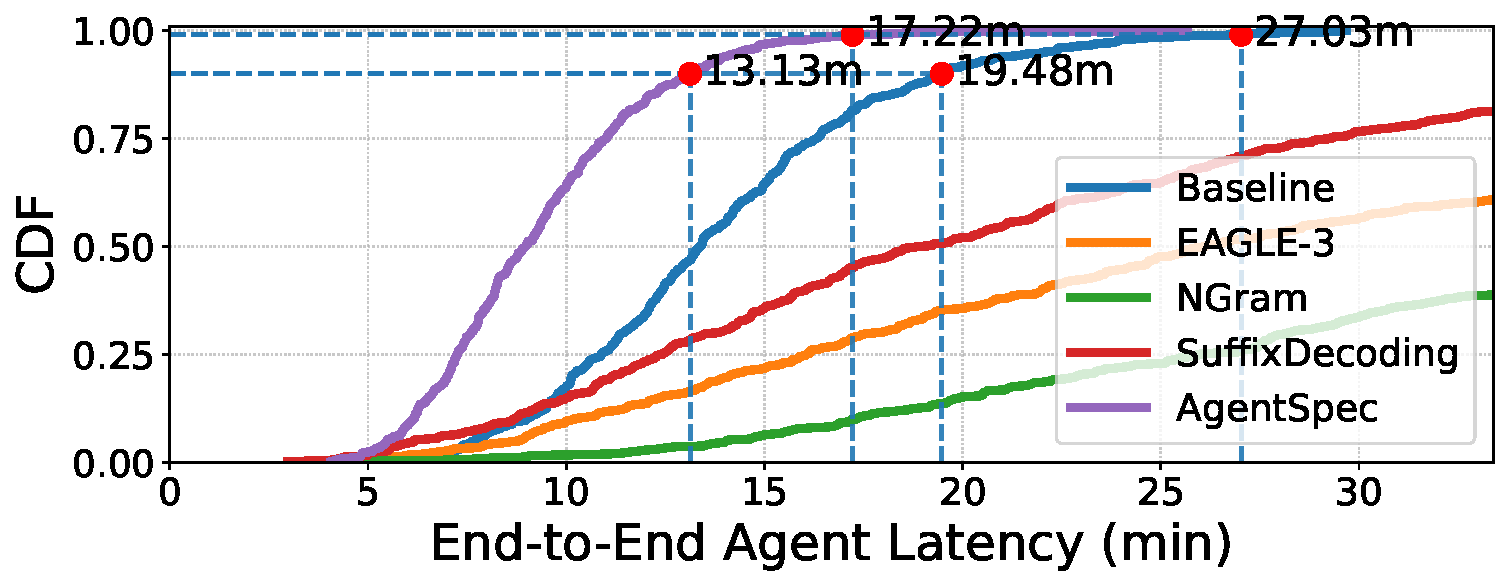
\includegraphics[width=0.48\textwidth]{Figures/e2e_latency.pdf}
\caption{Tailed latency analysis for \sysname and baselines on Code Gen agentic workflow.}
% \vspace{-3mm}
\label{fig:e2e_latency}
\end{figure}

% \begin{figure}[t]
% \centering
% \includegraphics[width=0.48\textwidth]{Figures/verification_cost.pdf}
% \caption{Drafting time cost for \sysname and baselines under different batch size.}
% % \vspace{-8mm}
% \label{fig:verification_cost}
% \end{figure}


\breakdownTable 

\subsection{Latency Analysis}
\label{subsec:tailed_latency_analysis} 
\noindent\textbf{Tailed Latency.} We further analyze the end-to-end program latency, defined as the time elapsed from when a user query is submitted to the agent application to when the final output is returned. The CDF of the tail latency is shown in~\cref{fig:e2e_latency}.
\sysname consistently achieves lower latency than baseline speculative decoding methods, and reduces tail latency by up to 1.47$\times$ and 1.39$\times$ compared to standard autoregressive decoding at the P90 and P99 percentiles, respectively.

\noindent\textbf{Execution Breakdown Analysis.}  We have performed fine-grained analysis including both drafting and verification costs on Reflexion Agentic Workflow. The results in~\cref{tab:runtime_breakdown} show that \sysname significantly reduces verification overhead compared to baselines, which is the dominant factor in overall speedup.  \sysname incurs slightly higher drafting overhead than NGram and SuffixDecoding. This additional cost mainly stems from maintaining the PDA in the structure-isolated drafting component and computing redundancy statistics in the redundancy-aware budget allocation module.
Nevertheless, the overhead remains negligible, amounting to less than 2 ms, and the overall drafting cost of \sysname is still lower than all baseline methods.


\subsection{Ablation Studies}
\label{subsec:ablation_study}
%
\sensitivityTable
% \acclenTable

\textbf{Modular Sensitivity Study.} We evaluate the separate contributions of the two key components (i.e., structure-isolated drafting and redundancy-aware budget allocation) of \sysname. 
%
Let \sysname \texttt{(S)} denote the version of \sysname with structure-isolated drafting only; \sysname \texttt{(R)} denote the version of \sysname with SuffixDecoding and redundancy-aware budget allocation.
%; and \sysname  denote the version of \sysname with both truncation-aware data whitening and parameter update with sequential low-rank approximation.
As shown in~\cref{tab:sensitivity}, we have three observations. 
%
(1) \sysname\texttt{(S)}, \sysname\texttt{(R)} and \sysname consistently outperform existing speculative decoding methods. 
%
(2) \sysname consistently outperforms both \sysname\texttt{(S)} and \sysname\texttt{(R)}.
%
This result demonstrates the unique contribution from each of the two key components and the importance of combining both components to achieve the best performance.
%
(3) Comparing between \sysname\texttt{(S)} and \sysname\texttt{(R)}, \sysname\texttt{(S)} achieves a higher speedup compared to \sysname\texttt{(R)}, indicating that structure-isolated drafting plays a more significant role than redundancy-aware budget allocation.

\noindent\textbf{Performance without Explicit Semantic Structures.} Since the structure-isolated drafting component of \sysname requires the agent application to provide explicit semantic block boundaries, some real-world agentic workloads may not expose such structure during generation. To assess the generality of \sysname, we have evaluated a variant that operates without semantic structure inputs, denoted as \sysname\texttt{(N)}. As shown in~\cref{tab:sensitivity}, \sysname\texttt{(N)} consistently outperforms both speculative decoding baselines and standard autoregressive decoding.
%Moreover,  We have instrumented vLLM to record the acceptance length at each verification step on the CodeGen agentic workload, and analyzed its distribution. We observe that while repetitive agentic template tokens exhibit slightly higher acceptance lengths than other tokens, they account for only a small portion of the overall generated tokens (8\% for Qwen-3-8B with thinking enabled). As a result, the average acceptance length over the full sequence remains close to that of non-template tokens. This indicates that the performance gains are not dominated by a small subset of repetitive agentic template tokens, but instead arise from consistent improvements across the majority of decoding steps.

\noindent\textbf{Performance Under Various Maximum Batch Size.} We next evaluate the performance of \sysname under different maximum batch size configurations in the vLLM engine. As shown in~\cref{fig:ablation}(a), while some existing speculative decoding methods (e.g., SuffixDecoding) achieve higher efficiency than standard autoregressive decoding at small batch sizes, their speedup gradually degrades and can even fall below autoregressive decoding as the maximum batch size increases.
In contrast, \sysname consistently maintains superior efficiency across all batch size configurations, outperforming both speculative decoding baselines and standard autoregressive decoding.

\begin{figure}[t]
\centering
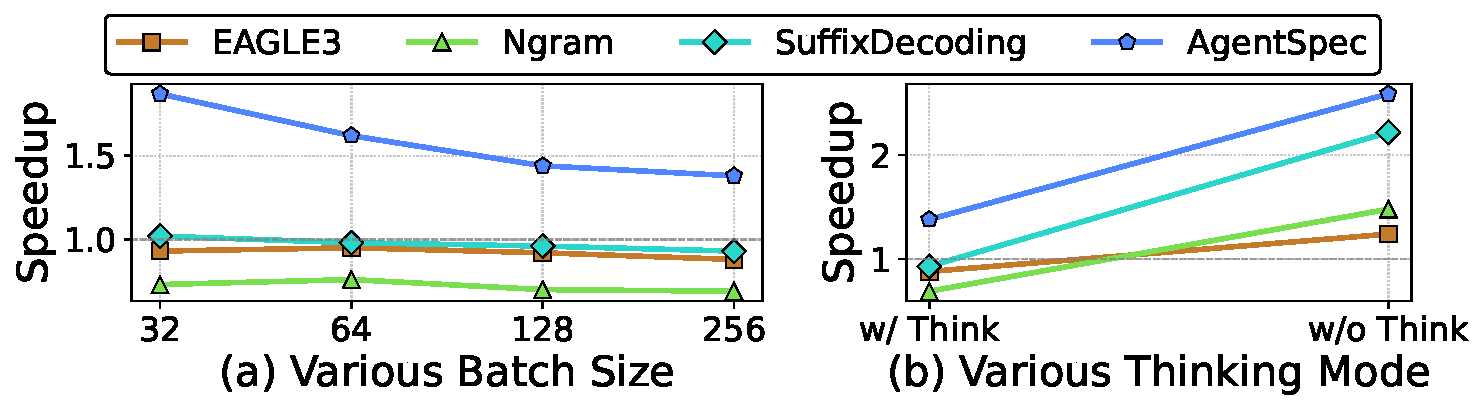
\includegraphics[width=\linewidth]{Figures/e2e_ablation.pdf}
\caption{Speedup in terms of Goodput (tokens/sec) of \sysname and baselines on workload of code generation agent under various maximum batch size and different thinking modes.}
\label{fig:ablation}
\end{figure}


\noindent\textbf{Performance in Different Thinking Modes.} Recent reasoning-oriented LLMs allow users to adjust thinking modes, which can substantially affect both the generated content and output length in agent applications.
To study this effect, we evaluate \sysname on Qwen-3-8B under two thinking modes: w/ think and w/o think~\citep{DBLP:journals/corr/abs-2505-09388}.
As shown in~\cref{fig:ablation}(b), \sysname consistently achieves superior performance across both modes. Notably, under the w/o think setting, \sysname is over 2.5$\times$ faster than standard autoregressive decoding.